\documentclass[12pt,a4paper]{article}
\usepackage{polski}
\usepackage[polish]{babel}
\usepackage{bbm}
\usepackage{bm}
\usepackage[T1]{fontenc}
\usepackage[utf8]{inputenc}
\usepackage[top=2cm, bottom=2cm, left=3cm, right=3cm]{geometry}
\usepackage{url}
\usepackage{graphics}
%\usepackage{graphicx}
\usepackage[pdftex]{graphicx}
\usepackage{float}
\usepackage{amsmath,amsthm}
\usepackage{enumitem}
\usepackage{epstopdf}
%\usepackage{indentfirst}
\usepackage[labelsep=period]{caption}
\setlist{nolistsep}

 

\AtBeginDocument{% Fragment zmieniający nazwy 'Rysunek' na 'Wykres' i 'Tablica' na 'Tabela'
        \renewcommand{\tablename}{Tabela}
        \renewcommand{\figurename}{Wykres}
}

\makeatletter
\newcommand{\linia}{\rule{\linewidth}{0.4mm}}

\let \savenumberline \numberline
\def \numberline#1{\savenumberline{#1.}}


\renewcommand*{\@seccntformat}[1]{%
	  \csname the#1\endcsname
		    .\quad
}



\floatstyle{plain}
\newfloat{image}{h!}{lop}
\floatname{image}{Rysunek}

\renewcommand{\maketitle}{\begin{titlepage}
		\vspace*{1cm}
    \begin{center}\small
    	Uniwersytet Wrocławski\\
    	Wydział Matematyki i Informatyki\\
    \end{center}
    \vspace{3cm}
    \noindent
    \linia
    \begin{center}
    	\LARGE{\textsc{\@title}}
         \end{center}
     \linia
    \begin{center}
    	\Large{Założenia wstępne}
         \end{center}
    \vspace{0.5cm}

    \begin{flushright}

    \begin{minipage}{5.5cm}

    	\small Autorzy:

    \normalsize {\@author} \par
    

    \end{minipage}
    \vspace{5cm}

     

     \end{flushright}

    \vspace*{\stretch{6}}

    \begin{center}

    \@date\\

    \end{center}

  \end{titlepage}%

}


\makeatother

\author{Jakub Stępniewicz (\textbf{233217})\\Dorota Suchocka (\textbf{233218})\\Radosław Warzocha (\textbf{123123})
\\Grupa {\bf XVII}}

\title{Do Domu\\ \small{Nawigator kieszonkowy}}


\begin{document}
\maketitle
\tableofcontents
\vspace{5cm}
	\begin{thebibliography}{9}
	%\bibitem{PE} P. Horowitz, W. Hill {\it Sztuka Elektroniki}, Warszawa 2009.
	\bibitem{MPK} \url{http://www.mpk.wroc.pl/}
	\bibitem{statystyki} \url{http://twojepc.pl/news27039.html}
	\bibitem{UE} \url{http://www.unrealengine.com/}
	\bibitem{GO} \url{http://www.google.pl/#sclient=psy-ab&hl=pl&source=hp&q=%22symulator+tramwaju+skoda+16t%22&pbx=1&oq=%22symulator+tramwaju+skoda+16t}
	\end{thebibliography}
\newpage
% 		Ok, najtrudniejsze za nami.		%
% 
\section{Wprowadzenie}
	\subsection{Cel dokumentu wizji}
	Celem niniejszego dokumentu jest opis wymagań stawianych aplikacji, ze względu na jej przeznaczenie, sposób użycia oraz najważniejszych założeń planu realizacji projektu. Temat implementacji nie jest tu podejmowany, zostanie on opisany w kolejnych dokumentach.
	
	\subsection{Ogólny opis produktu} 
	\textit{Do Domu} - aplikacja mobilna, ułatwiająca poruszanie się komunikacją miejską bez potrzeby posiadania połączenia z Internetem. \\ 

Podstawowym jej zadaniem będzie możliwość sprawdzenia najdogodniejszych połączeń tramwajów i autobusów należących do Miejskiego Przedsiębiorstwa Komunikacyjnego Sp. z o. o. we Wrocławiu. Dodatkowym usprawnieniem będzie możliwość wprowadzania ulubionych punktów w mieście, ma to przyspieszyć wyszukiwanie połączenia. W planach jest wprowadzenie nawigacji ułatwiającej zlokalizowanie kolejnych przystanków. \\ 

Każdy użytkownik będzie miał możliwość ujawnienia swojego położenia innym korzystającym z aplikacji.
	\newpage
	
\section{Opis użytkownika}

	\subsection{Dane statystyczne dot. użytkowników i rynku}
	Obecnie na rynku znajduje się bardzo niewiele rozwiązań tego typu, głównie są to rozwiązania wymagające połączenia z Internetem. \\
Zgodnie z szacowaniami z czerwca 2012 roku liczba użytkowników Androida wynosi około 380 milionów. Andy Rubin z firmy Google, główny pomysłodawca systemu operacyjnego Android, podał kilka statystyk dotyczących swojego dziecka. Według niego liczba dziennych aktywacji systemu przekroczyła już poziom 900 tysięcy \cite{statystyki}.	
	
	\subsection{Opis użytkowników }
	Aplikacja skierowana jest głównie do użytkowników połączeń Wrocławskiego Przedsiębiorstwa Komunikacyjnego \cite{MPK}. Nie jest jednak odrzucana możliwość poszerzenia bazy przez rozkłady innych przewoźników.

	\subsection{Środowisko użytkowników}
Potencjalni użytkownicy są w tej chwili zmuszeni korzystać z rozkładów znajdujących się na przystankach, co może być dla nich męczące i niewygodne, ponieważ znajdują się tam tylko rozkłady wybranych lini. \textit{Do Domu} ma na celu ułatwić im codzienne czynności związane z użytkowaniem sieci połączeń MPK.
	
	\subsection{Podstawowe potrzeby użytkownika }

Użytkownicy urządzeń mobilnych poszukują różnych rozwiązań ułatwiających im ich codzienne czynności, również te związane z poruszaniem się po mieście. Aplikacja będzie umożliwiała sprawne wyszukanie najlepszego połączenia, a także pokieruje podczas przesiadek.
	
	\subsection{Rozwiązania alternatywne i konkurencyjne}
	W tej chwili nie istnieją żadne rozwiązania konkurencyjne łączące wszystkie cechy, które chcemy osiągnąć w \textit{Do Domu}.
	\newpage

    \section{Ogólny opis produktu}

Z punktu widzenia użytkownika aplikacja ma być jego codziennym pomocnikiem w podróżowaniu po mieście. 

	\subsection{Schemat produktu}
	Główne elementy aplikacji: \\
	$\bullet$ połączenie GPS, \\
	$\bullet$ baza danych MPK, \\
	$\bullet$ algorytm wyszukiwania optymalnych połączeń, \\
	$\bullet$ intuicyjny graficzny interfejs użytkownika.	
 
	\subsection{Określenie pozycji produktu na rynku}
	
Aplikacja jest przeznaczona dla osób odczuwających potrzebę wygodniejszego planowania wyjazdów oraz chcących mieć możliwość sprawdzenia połączeń MPK w każdej sytuacji. \\ 

Produkt na pewno znajdzie swoje miejsce na rynku, ponieważ wyraźnie brakuje aplikacji, która umożliwia sprawdzenie offline różnych wariantów podróży. Do tego wielkim udogodnieniem jest możliwość dodawania głównego celu trasy oraz innych ulubionych punków, do których użytkownik podróżuje tj. miejsce pracy, uczelnia.

	\subsection{Założenia i zależności}	
	
Zakładamy że użytkownik aplikacji nie dysponuje dużą wiedzą informatyczną, dlatego też interfejs \textit{Do Domu} powinien być intuicyjny i łatwy w obsłudze, aby można było w łatwy sposób uzyskać dostęp do wszystkich funkcjonalności systemu.

\newpage

\section{Cechy produktu}

	\subsection{Kontrola długów osobistych}

System umożliwia sprawdzenie zadłużenia w ramach jednego użytkownika i w zależności od wysokości długu sugeruje oszczędność.

	\subsection{Możliwość tworzenia grup w ramach których widać wzajemne długi}

Do grupy mają dostęp wszyscy użytkownicy do niej należący. Każdy z nich może przeglądać historię zmian dokonanych przez innych członków grupy.

	\subsection{Możliwość sprawdzenia cudzego balansu}

W ramach członków grupy istnieje możliwość sprawdzenia cudzego zadłużenia w celu generowania statystyk, co pomoże w określeniu wiarygodności dłużnika.

	\subsection{Plan spłat}

System umożliwia stworzenie kalendarza spłat i zwrotów. Dzięki czemu wspomaga podjęcie decyzji o oszczędzaniu lub próbie rozłożenia spłat na dłużysz okres.

	\subsection{Integracja z portalem społecznościowym}

Moduł “wydarzenia” pozwala na sprawdzenie salda w ramach wydarzeń ogłaszanych na portalu społecznościowym.

	\subsection{Wspólne zakupy}

Moduł umożliwiający dodanie jednego wpisu, w którym będzie zawarta kwota, osoba płacąca oraz dane uczestników wspólnych zakupów.

	\subsection{Redukcja długów}

System umożliwia redukowanie długów zamkniętych w cykle i w zależności od preferencji użytkowników istnieje opcja skrócenia ścieżki zadłużenia pomiędzy członkami grupy.

	\subsection{Wersja mobilna}

Aplikacja, którą można zainstalować na własnym telefonie w celu bieżącej aktualizacji zadłużenia.

\newpage

\section{Cechy produktu}
\subsection{W pełni odzwierciedlony kokpit tramwaju \textit{Škoda 19T}}
Podstawowym elementem symulatora jest wymodelowane z największą dokładnością miejce pracy motorniczego. Składa się ono z licznych przełączników, dwóch ekranów ciekłokrystalicznych oraz \textbf{przepustnicy} sterującej prędkością tramwaju. Całość będzie obsługiwana
przez osobny system wbudowany działający na mikroprocesorach typu \textit{ATmega128}.

Poglądowy wygląd kokpitu przedstawiony został na rysunku \ref{cock}.

\begin{image}
	\begin{center}
		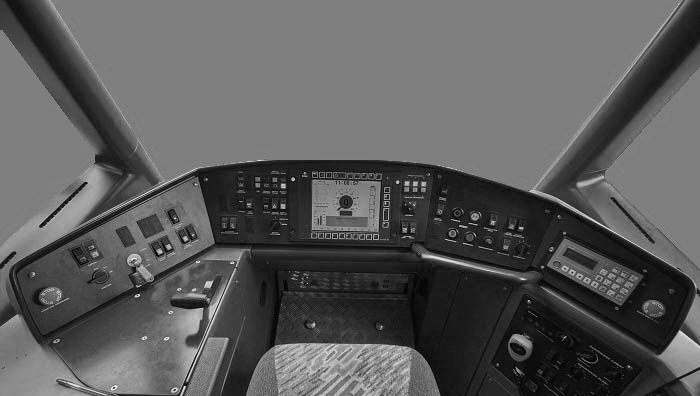
\includegraphics[bb=0 0 700px 396px]{img/cockBW.jpg}
		\caption{Kokpit tramwaju {\it Škoda 19T}}
			\label{cock}
	\end{center}
\end{image}

\subsection{Realistyczne środowisko symulacyjne}
Sercem symulacji jest program komputerowy odzwierciedlający działanie wcześniej wspominanego tramwaju. Wysoka jakość grafiki
zostanie zapewniona przez silnik \textit{Unreal Engine 3}\cite{UE}. Program będzie się komunikował za pomocą specjalnego protokołu z mikrokontrolerem,
co umożliwi szybkie przekazanie wszystkich paramatrów pojazdu do kokpitu.
	\newpage
	
\section{Podstawowe przypadki użycia}
Podstawowym zadaniem symulatora jest umożliwienie motorniczym, oraz kandydatom na motorniczego przećwiczenie zachowań w trudnych sytuacjach drogowych. Pozwala on także przyzwyczaić kandydatów na motorniczych do nowego systemu sterowania zastosowanego w tym tramwaju. Wiernie odwzorowane otoczenie dostarczy podstawowego obrazu pracy obsługi pojazdu trakcyjnego.
	\newpage
	
\section{Wymagania dokumentacyjne}
\subsection{Pomoc techniczna}
Elementem symulatora będzie bezpłatny, roczny okres pełnej pomocy technicznej, dostępnej 24 godziny na dobę, 7 dni w tygodniu. Każda usterka sprzętu i oprogramowania będzie naprawiana w najwcześniejszym możliwym terminie.

\subsection{Instalacja i konfiguracja}
Producent sprzętu i oprogramowania zapewnia zainstalowanie sprzętu w wybranym przez klienta miejscu. Instalacja obejmuje przeszkolenie personelu niezbędnego do obsługi symulatora (instruktor).

\subsection{Oznaczenia i pakowanie}
Symulator jest dostarczany w 11 kartonowych opakowaniach. Zawartość poszczególnych opakowań została przedstawiona w tabeli \ref{elem} na stronie \pageref{elem}.

\begin{table}[h]
\caption{Pakowanie elementów}
	\begin{center}
\begin{tabular}{l|l}
\texttt{Element} & \texttt{Numer opakowania} \\ \hline
Komputer osobisty odpowiedzialny za symulację & KX7004 \\
Ekrany ciekłokrystaliczne kokpitu & KX1201 \\
Przełączniki i przepustnica kokpitu& KX1202 \\
Fotel motorniczego & KX1203 \\
Okablowanie kokpitu & KX1204 \\
Mikrokontrolery odpowiedzialne za sterowanie & KX1205 \\
Elementy plastikowe kokpitu cz. I & KX1206 \\
Elementy plastikowe kokpitu cz. II & KX1207 \\
Urządzenia peryferyjne stanowiska instruktora & KX4401 \\
Oprogramowanie symulatora & KX6635 \\
Kolorowy dywanik & KX2266
\end{tabular}
\label{elem}
\end{center}
\end{table}

\end{document}

